\documentclass{article}
\usepackage[utf8]{inputenc}
\usepackage[margin=1in]{geometry}

\title{481 - Homework 11}
\author{Victor Zhang}
\date{November 27, 2020}

\usepackage[utf8]{inputenc}
\usepackage{amsmath}
\usepackage{amsfonts}
\usepackage{natbib}
\usepackage{graphicx}
% \usepackage{changepage}
\usepackage{amssymb}
\usepackage{xfrac}
% \usepackage{bm}
% \usepackage{empheq}
\usepackage{tikz}
\usepackage{pgfplots}

\newcommand{\contra}{\raisebox{\depth}{\#}}

\newenvironment{myindentpar}[1]
  {\begin{list}{}
          {\setlength{\leftmargin}{#1}}
          \item[]
  }
  {\end{list}}

\pagestyle{empty}

\begin{document}

\maketitle
% \begin{center}
% {\huge Econ 482 \hspace{0.5cm} HW 3}\
% {\Large \textbf{Victor Zhang}}\
% {\Large February 18, 2020}
% \end{center}

\section*{12.17}
\subsection*{12.17.1}
For the hypergeometric, $X \geq k$, so $Pr(X = 2 \;|\; k=0) = Pr(X=2 \;|\; k=1) = 0$. $Pr(X = 2 \;|\; k=2) = \frac{\binom{2}{2}\binom{5}{0}}{\binom{7}{2}} = \frac{1}{21}$. Then $\alpha_{k=0} = \alpha_{k=1} = 0$ and $\alpha_{k=2} = \frac{1}{21}$ $\Box$

\subsection*{12.17.2}
$Pr(X = 2 \;|\; k = 4) = \frac{\binom{4}{2}\binom{3}{0}}{\binom{7}{2}} = \frac{2}{7}$, $Pr(X = 2 \;|\; k = 5) = \frac{\binom{5}{2}\binom{2}{0}}{\binom{7}{2}} = \frac{10}{21}$, $Pr(X = 2 \;|\; k = 6) = \frac{\binom{6}{2}\binom{1}{0}}{\binom{7}{2}} = \frac{5}{7}$, $Pr(X = 2 \;|\; k = 7) = \frac{\binom{7}{2}\binom{0}{0}}{\binom{7}{2}} = 1$. Then $\beta_{k=4} = \frac{5}{7}$, $\beta_{k=5} = \frac{11}{21}$, $\beta_{k=6} = \frac{2}{7}$, $\beta_{k=7} = 0$ $\Box$
\begin{figure}[ht]
\centering
\begin{tikzpicture}
\begin{axis}[
    xlabel={k},
    ylabel={Power},
    xmin=3, xmax=8,
    ymin=0, ymax=1,
    xtick={4,5,6,7},
    ytick={0.0,0.2,0.4,0.6,0.8,1.0},
    ymajorgrids=true,
    grid style=dashed,
]
\addplot[
    color=blue,
    mark=square,
    ]
    coordinates {
    (4,0.285714)(5,0.476190)(6,0.7142857)(7,1)
    };
\end{axis}
\end{tikzpicture}
\end{figure}

\section*{12.18}
We calculate $\pi(\theta) = Pr(\text{reject } H_0 \;|\;\theta) = Pr(X \leqslant 15 \;|\; \theta) = \sum\limits_{k=0}^{15} \binom{20}{k}\theta^k(1-\theta)^{20-k}$
\begin{figure}[ht]
\centering
\begin{minipage}{.5\textwidth}
  \begin{center}
  \begin{tabular}{ c|c }
  $\theta$ & $\pi(\theta)$\\
  \cline{1-2}
  0.95 & 0.00257\\
  0.90 & 0.04317\\
  0.85 & 0.17015\\
  0.80 & 0.37035\\
  0.75 & 0.58516\\
  0.70 & 0.76249\\
  0.65 & 0.88180\\
  0.60 & 0.94905\\
  0.55 & 0.98114\\
  0.50 & 0.99409\\
  \end{tabular}
  \end{center}
  \label{fig:test1}
\end{minipage}%
\begin{minipage}{.5\textwidth}
  \centering
  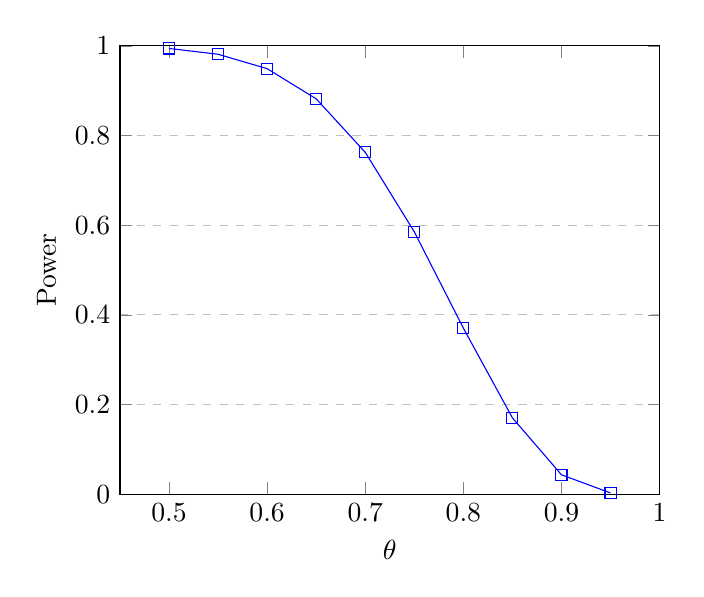
\begin{tikzpicture}
\begin{axis}[
    xlabel={$\theta$},
    ylabel={Power},
    xmin=0.45, xmax=1.0,
    ymin=0, ymax=1,
    xtick={0.5,0.6,0.7,0.8,0.9,1.0},
    ytick={0.0,0.2,0.4,0.6,0.8,1.0},
    ymajorgrids=true,
    grid style=dashed,
]
\addplot[
    color=blue,
    mark=square,
    ]
    coordinates {
    (0.95,0.00257)(0.90,0.04317)(0.85,0.17015)(0.80,0.37035)(0.75,0.58516)(0.70,0.76249)(0.65,0.88180)(0.60,0.94905)(0.55,0.98114)(0.50,0.99409)
    };
\end{axis}
\end{tikzpicture}
  \label{fig:test2}
\end{minipage}
\caption{Table and plot for problem 12.18}
\end{figure}

\section*{12.19}
$\max L_0$ follows from the fact that our hypothesis is simple. $L$ is maximized by putting $\mu = \overline{x}$, the maximum-likelihood estimator for $\mu$. Since $\overline{x} \in H_1$, we may conclude $\max\limits_{H_1} L$ is achieved at $\mu = \overline{x}$. Next recall the identity
$$\sum (x_i - \mu)^2 = \sum (x_i - \overline{x})^2 + n(\overline{x}-\mu)^2$$
which was established in the sketch of the proof that $\frac{(n-1)s^2}{\sigma^2} \sim \chi^2_{n-1}$ if $X_i$ normal. The desired result is immediate from properties of dividing exponents $\Box$

\section*{12.20}
\subsection*{12.20.1}
Since $H_0$ is simple, $L_0(x) = \binom{n}{x} \left(\frac{1}{2}\right)^x \left(\frac{1}{2}\right)^{n-x}$. The MLE estimator of $\theta$ is $x$, so $L_1 = \binom{n}{x} \left(\frac{x}{n}\right)^x \left(\frac{n-x}{n}\right)^{n-x}$. Then
$$\lambda = \frac{\binom{n}{x} \left(\frac{1}{2}\right)^x \left(\frac{1}{2}\right)^{n-x}}{\binom{n}{x} \left(\frac{x}{n}\right)^x \left(\frac{n-x}{n}\right)^{n-x}} = \left(\frac{n/2}{x} \right)^x \left(\frac{n/2}{n-x}\right)^{n-x} \leqslant K \; \Box$$

\subsection*{12.20.2}
By monotonicity of $\ln$, we may express the critical region as
\begin{gather*}
\ln\lambda = x\ln(n/2) - x\ln x + (n-x)\ln(n/2) - (n-x)\ln(n-x) \leqslant C_1\\
n\ln(n/2) - x\ln x - (n-x)\ln(n-x) \leqslant C_1\\
- x\ln x - (n-x)\ln(n-x) \leqslant C_2\\
x\ln x + (n-x)\ln(n-x) \geqslant K
\end{gather*}
where $C_1, C_2, K$ are constants $\Box$

\subsection*{12.20.3}
For any given value of $n$, $f$ is symmetric about $n/2$ with a minimum exactly at $x = n/2$. Thus, the critical region may be written as $|x-\frac{n}{2}| \geqslant K$ for some constant $K$ $\Box$

\section*{12.21}
\subsection*{12.21.1}
Since $H_0$ is simple, we may write $L_0 = \left(\frac{1}{\theta_0}\right)^n e^{-\sum x_i / \theta_0}$. The MLE estimator is $\theta = \overline{x}$ so we may write $L_1 = \left(\frac{1}{\overline{x}}\right)^n e^{-\sum x_i / \overline{x}}$. Then
$$\lambda = \frac{\left(\frac{1}{\theta_0}\right)^n e^{-\sum x_i / \theta_0}}{\left(\frac{1}{\overline{x}} \right)^n e^{-\sum x_i / \overline{x}}} = \left(\frac{\overline{x}}{\theta_0}\right)^n e^{n - \sfrac{n\overline{x}}{\theta_0}} \leqslant K \; \Box$$

\subsection*{12.21.2}
By monotonicity of $\log$
\begin{gather*}
\ln\lambda = n\ln \overline{x} - n\ln \theta_0 + n - n\frac{\overline{x}}{\theta_0} \leqslant C_1\\
\ln\overline{x} - \frac{\overline{x}}{\theta_0} \leqslant C_2\\
\overline{x}e^{-\overline{x}/\theta_0} \leqslant K
\end{gather*}
as desired $\Box$

\section*{12.22}
Recall the joint MLE estimators of $\mu$ and $\sigma^2$ are $\overline{x}$ and ${s'}^2$, respectively. From the derivation of example 10.17, we may conclude the MLE of $\sigma^2$ under restriction $\mu = \mu_0$ to be $\frac{\sum(x_i-\mu_0)^2}{n}$.
Given $\mu = \mu_0$, $\max\limits_{\sigma^2} L_0 = \frac{1}{\sqrt{2\pi\sum(x_i-\mu_0)^2/n}^n}e^{-n/2}$. Without this restriction on $\mu$, $\max\limits_{\mu,\sigma^2} L = \frac{1}{\sqrt{2\pi\sum(x_i-\overline{x})^2/n}^n}e^{n/2}$. Then
\begin{equation*}
\begin{split}
\lambda = \frac{\frac{1}{\sqrt{2\pi\sum(x_i-\mu_0)^2/n}^n}e^{n/2}}{\frac{1}{\sqrt{2\pi\sum(x_i-\overline{x})^2/n}^n}e^{n/2}} &= \left(\frac{\sum(x_i-\overline{x})^2}{\sum(x_i-\mu_0)^2}\right)^{n/2} = \left(\frac{\sum(x_i-\mu_0)^2}{\sum(x_i-\overline{x})^2}\right)^{-n/2}\\
&= \left(\frac{\sum(x_i-\overline{x})^2 + n(\overline{x}-\mu_0)^2}{\sum(x_i-\overline{x})^2}\right)^{-n/2}\\
&= \left(1 + \frac{n(\overline{x}-\mu_0)^2}{(n-1)s^2}\right)^{-n/2}\\
&= \left(1+ \frac{\left(\frac{\overline{x}-\mu_0}{s/\sqrt{n}}\right)^2}{n-1}\right)^{-n/2} \leqslant K
\end{split}
\end{equation*}
as desired $\Box$

\section*{12.23}
$$-2\ln\lambda = n\ln\left(1+\frac{t^2}{n-1}\right)$$
We note for small $x$ that $\ln(1+x) \approx x$, justifying this by recalling the Taylor expansion
$$\ln(1+x) = x - \frac{x^2}{2} + \frac{x^3}{3} \dots$$
Then $\lim\limits_{n\rightarrow \infty} n\ln\left(1+\frac{t^2}{n-1}\right) = \lim\limits_{n\rightarrow\infty} \frac{n}{n-1}t^2 = t^2$ $\Box$

\section*{12.24}
We observe in example 10.17 that the derivation of the MLE for $\mu$ does not involve $\sigma$ at all. Then in both likelihood functions we may put $\mu = \overline{x}$. Since the function $f(x) = x^2$ is monotonically increasing on $x \geqslant 0$, we can derive the MLE estimator of $\sigma$ from the MLE estimator of $\sigma^2$ as exactly $\sqrt{{s'}^2} = s'$
$$\lambda = \frac{\left(\frac{1}{2\pi\sigma_0^2}\right)^{-n/2}e^{-\sum(x_i-\overline{x})^2/2\sigma_0^2}}{\left(\frac{1}{2\pi{s'}^2}\right)^{-n/2}e^{-\sum(x_i-\overline{x})^2/2{s'}^2}} = \left(\frac{s'}{\sigma_0}\right)^{-n} e^{n/2(1 - {s'}^2/\sigma_0^2)} \leqslant K \;\Box$$

\section*{12.25}
\subsection*{12.25.1}
The likelihood function is given by
$$L(\vec{x}, \vec{\mu}, \vec{\sigma}^2) = \prod\limits^k (2\pi\sigma_i^2)^{-n_i/2} e^{-\sum\limits^j(x_{ij}-\mu_i)^2/2\sigma_i^2}$$
Similarly to example 10.17 we may find maximizers $\mu_i = \overline{x}_i$ independent of all other parameters. Then the likelihood function becomes
$$L(\vec{x},\vec{\sigma}^2) = \prod\limits^k (2\pi\sigma_i^2)^{-n_i/2} e^{-\sum\limits^j(x_{ij}-\overline{x}_i)^2/2\sigma_i^2} = \prod\limits^k (2\pi\sigma_i^2)^{-n_i/2} e^{-(n_i-1)s_i^2/2\sigma_i^2}$$
Under $H_0$,
\begin{gather*}
L(\vec{x},\sigma^2) =(2\pi\sigma^2)^{-n/2} e^{-\sum(n_i-1)s_i^2 /2\sigma^2}\\
\ln L(\vec{x},\sigma^2) = -\frac{n}{2}\ln(2\pi\sigma^2)-\frac{\sum(n_i-1)s_i^2}{2\sigma^2}\\
\frac{\partial}{\partial\sigma^2}\ln L(\vec{x},\sigma^2) = -\frac{n}{2\sigma^2}+\frac{\sum(n_i-1)s_i^2}{2\sigma^4}
\end{gather*}
Setting the partial derivative to zero, we see $L$ is maximized when $\sigma^2_i = \sigma^2 = \frac{\sum(n_i-1)s_i^2}{n}$.\\
Althernatively,
\begin{gather*}
L(\vec{x},\vec{\sigma}^2) = \prod\limits^k (2\pi\sigma_i^2)^{-n_i/2} e^{-(n_i-1)s_i^2/2\sigma_i^2}\\
\ln L(\vec{x},\vec{\sigma}^2) = \sum\limits^k -\frac{n}{2}\ln(2\pi\sigma_i^2)-\frac{\sum(n_i-1)s_i^2}{2\sigma_i^2}\\
\frac{\partial}{\partial\sigma_i^2}\ln L(\vec{x},\vec{\sigma}^2) = -\frac{n_i}{2\sigma_i^2} + \frac{(n_i-1)s_i^2}{2\sigma_i^4}
\end{gather*}
Setting the partial derivative to zero, we see $L$ is maximized when $\sigma_i^2 = \frac{(n_i-1)s^2}{n}$ $\Box$

\subsection*{12.25.2}
Plugging the derived MLE estimators into the likelihood functions,
$$\lambda = \frac{L_0}{L_1} = \frac{(2\pi\frac{\sum(n_i-1)s_i^2}{n})^{-n/2} e^{-n/2}}{\prod\limits^k (2\pi\frac{(n_i-1)s_i^2}{n_i})^{-n_i/2} e^{-n_i/2}} = \frac{\prod \left[\frac{(n_i-1)s_i^2}{n_i}\right]^{n_i/2}}{\left[\sum \frac{(n_i-1)s_i^2}{n}\right]^{n/2}} \; \Box$$

\section*{12.26}
Divide both sides by $(s_1^2)^{n/2}$ to get
$$\lambda = \frac{\left(\frac{(n_1-1)s_1^2}{n_1}\right)^{n_1/2} \left(\frac{(n_2-1)s_2^2}{n_2}\right)^{n_2/2}}{\left(\frac{(n_1-1)s_1^2 + (n_2-1)s_2^2}{n}\right)^{n/2}} = \frac{\left(\frac{n_1-1}{n_1}\right)^{n_1/2}\left(\frac{(n_2-1)}{n_2}\frac{s_2^2}{s_1^2}\right)^{n_2/2}}{\left(\frac{(n_1-1)}{n}+\frac{(n_2-1)}{n}\frac{s_2^2}{s_1^2}\right)^{n/2}} \; \Box$$

\section*{12.27}
$X$ has a uniform distribution under $H_0$ so trivially the critical region has size $\alpha$.
$$Pr(\textrm{reject } H_0 \;|\; \theta) = \int\limits_0^\alpha 1 + \theta^2(\frac{1}{2}-x)\;\mathrm{d}x = x\left(1+\frac{\theta^2}{2}\right)-\frac{\theta^2}{2}x^2 \Big\vert_0^\alpha = \alpha + \frac{\theta^2}{2}(\alpha-\alpha^2)$$
Since $\alpha < 1$, $\alpha - \alpha^2 > 0$ and the probability of rejecting $H_0$ is decreasing in $\theta^2$. Then the power is minimized when $\theta = 0$, and the critical region is unbiased $\Box$

\section*{13.1}
The standard two-sided test criterion is $\left\vert\frac{\overline{X}-\mu_0}{\sigma/\sqrt{n}}\right\vert > z_{\alpha/2}$. But $Z^2 = \chi^2_1$ so we may transform this test criterion into
$$\left(\frac{\overline{X}-\mu_0}{\sigma/\sqrt{n}}\right)^2 > \chi^2_{1,\alpha} \; \Box$$

\section*{13.2}
We will use a one-sided test.\\
$Pr(\frac{\overline{X}-\mu_0}{\sigma/\sqrt{n}} > z_\alpha) = \alpha$. Then the critical region may be expressed as
$$C : \{\overline{X} \geqslant \mu_0 + \frac{\sigma}{\sqrt{n}}z_\alpha\}$$
$Pr(\frac{\overline{X}-\mu_1}{\sigma/\sqrt{n}} < -z_\beta) = \beta$. Then the critical region may be expressed as
$$C : \{\overline{X} \geqslant \mu_1 - \frac{\sigma}{\sqrt{n}}z_\beta\}$$
Equating $\mu_0 + \frac{\sigma}{\sqrt{n}}z_\alpha = \mu_1 - \frac{\sigma}{\sqrt{n}}z_\beta$ yields the desired result $\Box$

\section*{13.3}
$$n = \frac{\sigma^2(z_\alpha+z_\beta)^2}{(\mu_1-\mu_0)^2} = \frac{9^2\cdot(1.64+2.33)^2}{(20-15)^2} = 51.06 \approx 52 \Box$$

\section*{13.4}
WLOG suppose $\delta' > \delta$. From the calculations we will see the case where $\delta' < \delta$ may be treated similarly with the same results. We use the one-sided test. Denote by $\sigma^2/n$ the variance of the difference of sample means, given $\sigma^2/n = \frac{\sigma^2_1 + \sigma^2_2}{n}$\\
$Pr(\frac{(\overline{X}_1-\overline{X}_2) - \delta}{\sigma/\sqrt{n}} > z_\alpha) = \alpha$. So the critical region may be written
$$C : \{\overline{X}_1-\overline{X}_2 \geqslant \delta + \frac{\sigma}{\sqrt{n}}z_\alpha \}$$
$Pr(\frac{(\overline{X}_1-\overline{X}_2) - \delta'}{\sigma/\sqrt{n}} < -z_\beta) = \beta$. So the critical region may be written
$$C : \{\overline{X}_1-\overline{X}_2 \geqslant \delta' - \frac{\sigma}{\sqrt{n}}z_\beta \}$$
Equating $\delta + \frac{\sigma}{\sqrt{n}}z_\alpha = \delta' - \frac{\sigma}{\sqrt{n}}z_\beta$ yields the desired result $\Box$

\section*{13.5}
$$n = \frac{(\sigma^2_1+\sigma^2_2)(z_\alpha+z\beta)^2}{(\delta-\delta')^2} = \frac{(9^2+13^2)(2.33+2.33)^2}{(80-86)^2} = 150.80 \approx 151 \; \Box$$

\section*{13.6}
$\frac{(n-1)s^2}{\sigma^2} \sim \chi^2_{n-1}$ if $X_i$ i.i.d. Normal. $\frac{\chi^2_n - n}{\sqrt{2n}} \sim Z$ for large $n$. Then
$$\frac{\frac{(n-1)s^2}{\sigma^2} - (n-1)}{\sqrt{2(n-1)}} = \frac{\frac{s^2}{\sigma^2}-1}{\sqrt{\frac{2}{n-1}}} \sim Z$$
Then $Pr(\frac{\sfrac{s^2}{\sigma^2_0}-1}{\sqrt{\frac{2}{n-1}}} > z_\alpha) = \alpha$. The critical region is thus $C : \{s^2 \geqslant \sigma^2_0 \left[1+z_\alpha\sqrt{\frac{2}{n-1}}\;\right]\}$, as desired.\\
If instead we used the alternative hypothesis $H_1: \sigma^2 < \sigma_0^2$, we would write $Pr(\frac{\sfrac{s^2}{\sigma^2_0}-1}{\sqrt{\frac{2}{n-1}}} < -z_\alpha) = \alpha$ and the critical region would be $C : \{s^2 \leqslant \sigma^2_0 \left[1-z_\alpha\sqrt{\frac{2}{n-1}}\;\right]\}$.\\
If we used $H_1: \sigma^2 \neq \sigma^2_0$, we would write $Pr(\left\vert\frac{\sfrac{s^2}{\sigma^2_0}-1}{\sqrt{\frac{2}{n-1}}}\right\vert > z_{\alpha/2}) = \alpha$ and get critical region $C : \{|s^2 - \sigma^2_0| \geqslant z_{\alpha/2}\sqrt{\frac{2}{n-1}}\}$ $\Box$

\section*{13.7}
We typically use the fact $\frac{(n-1)s^2}{\sigma^2} \sim \chi^2_{n-1}$. Since $\sqrt{2\chi^2_n}-\sqrt{2n} \sim Z$, we may say
$$\sqrt{\frac{2(n-1)s^2}{\sigma^2}} -\sqrt{2(n-1)} = \left(\frac{s}{\sigma_0}-1\right)\sqrt{2(n-1)} \sim Z \;\Box$$

\section*{13.8}
It suffices to show
$$\frac{(x_i-n_i\hat{\theta})^2}{n_i\hat{\theta}(1-\hat{\theta})} = \sum\limits_{j=1}^{2}\frac{(f_{ij}-e_{ij})^2}{e_{ij}}$$
Behind the jargon, $e_{i1} = n_i\hat{\theta}$, $e_{i2} = n_i(1-\hat{\theta})$, $f_{i1} = x_i$, $f_{i2} = n_i - x_i$. Then
\begin{equation*}
\begin{split}
\sum\limits_{j=1}^{2}\frac{(f_{ij}-e_{ij})^2}{e_{ij}} &= \frac{(x_i-n_i\hat{\theta})^2}{n_i\hat{\theta}} + \frac{((n_i-x_i)-n_i(1-\hat{\theta}))^2}{n_i(1-\hat{\theta})}\\
&= \frac{(x_i-n_i\hat{\theta})^2}{n_i\hat{\theta}} + \frac{(n_i\hat{\theta}-x_i)^2}{n_i(1-\hat{\theta})}\\
&= \frac{(x_i-n_i\hat{\theta})^2}{n_i}\left(\frac{1}{\hat{\theta}}+\frac{1}{1-\hat{\theta}} \right)\\
&= \frac{(x_i-n_i\hat{\theta})^2}{n_i\hat{\theta}(1-\hat{\theta})}
\end{split}
\end{equation*}
as desired $\Box$

\section*{13.9}
Recall the sum of independent Poisson variables with parameters $\lambda_1$ and $\lambda_2$ results in a Poisson variable with parameter $\lambda_1+\lambda_2$. Then $\sum\limits^n X_i \sim Pois(n\lambda)$. The critical region for $H_1 : \lambda > \lambda_0$ is $\{\sum X_i \geqslant k_{n\lambda_0,\alpha}\}$. The critical region for $H_1 : \lambda < \lambda_0$ is $\{\sum X_i \leqslant k'_{n\lambda_0,\alpha}\}$. The critical region for $H_1 : \lambda \neq \lambda_0$ is $\{\sum X_i 
\leqslant k'_{n\lambda_0, \alpha/2} \textrm{ or } \sum X_i \geqslant k_{n\lambda_0, \alpha/2} \}$ $\Box$

\section*{13.10}
$n\lambda_0 = 5\cdot3.6 = 18$. $k_0.025 = 25$ and $k'_0.025 = 9$. So we reject if $\overline{X} \geqslant 25$ or $\overline{X} \leqslant 9$ $\Box$

\section*{13.11}
\begin{equation*}
\begin{split}
\chi^2 &= \frac{(x_1-n_1\hat{\theta})^2}{n_1\hat{\theta}(1-\hat{\theta})} + \frac{(x_2-n_2\hat{\theta})^2}{n_2\hat{\theta}(1-\hat{\theta})}\\
&= \frac{(x_1-\frac{n_1(x_1+x_2)}{n_1+n_2})^2}{n_1\hat{\theta}(1-\hat{\theta})} + \frac{(x_2-\frac{n_2(x_1+x_2)}{n_1+n_2})^2}{n_2\hat{\theta}(1-\hat{\theta})}\\
&= \frac{(\frac{x_1n_2-x_2n_1}{n_1+n_2})^2}{n_1\hat{\theta}(1-\hat{\theta})} + \frac{(\frac{x_2n_1-x_1n_2}{n_1+n_2})^2}{n_2\hat{\theta}(1-\hat{\theta})}\\
&= \frac{(n_1+n_2)(\frac{x_1n_2-x_2n_1}{n_1+n_2})^2}{n_1n_2\hat{\theta}(1-\hat{\theta})}\\
&= \frac{\frac{(x_1n_2-x_2n_1)^2}{n_1+n_2}}{n_1n_2\frac{x_1+x_2}{n_1+n_2}\frac{n_1+n_2-x_1-x_2}{n_1+n_2}}\\
&= \frac{(n_1+n_2)(x_1n_2-x_2n_1)^2}{n_1n_2(x_1+x_2)[(n_1+n_2)-(x_1+x_2)]} \; \Box
\end{split}
\end{equation*}

\section*{13.12}
For large samples, we may use the normality approximation. That is, $x_i \sim N(n_i\theta_i, n_i\theta_i(1-\theta_i))$ so $\frac{x_i}{n_i} \sim N(\theta_i, \frac{\theta_i(1-\theta_i)}{n_i})$. Under assumption that $\theta_1 = \theta_2$ we may pool proportions as $\hat{\theta} = \frac{x_1+x_2}{n_1+n_2}$. Then by the test statistic for difference of means of Normal populations,
$$\frac{\frac{x_1}{n_1}-\frac{x_2}{n_2}}{\sqrt{\hat{\theta}(1-\hat{\theta})\left(\frac{1}{n_1}+\frac{1}{n_2}\right)}} \sim Z$$
as desired $\Box$

\section*{13.13}
\begin{equation*}
\begin{split}
\left[\frac{\frac{x_1}{n_1}-\frac{x_2}{n_2}}{\sqrt{\hat{\theta}(1-\hat{\theta})\left(\frac{1}{n_1}+\frac{1}{n_2}\right)}}\right]^2 &= \frac{\left(\frac{x_1n_2-x_2n_1}{n_1n_2}\right)^2}{\hat{\theta}(1-\hat{\theta})\left(\frac{n_1+n_2}{n_1n_2}\right)}\\
&= \frac{(x_1n_2-x_2n_1)^2}{n_1n_2(n_1+n_2)\hat{\theta}(1-\hat{\theta})}\\
&= \frac{(x_1n_2-x_2n_1)^2}{n_1n_2(n_1+n_2)\frac{x_1+x_2}{n_1+n_2}\frac{(n_1+n_2)-(x_1+x_2)}{n_1+n_2}}\\
&= \frac{(n_1+n_2)(x_1n_2-x_2n_1)^2}{n_1n_2(x_1+x_2)[(n_1+n_2)-(x_1+x_2)]}
\end{split}
\end{equation*}
From exercise 11, this is exactly $\chi^2 = \sum\limits^2_{i=1} \frac{(x_i-n_i\hat{\theta})^2}{n_i\hat{\theta}(1-\hat{\theta})}$, so we are done $\Box$


\end{document}

% List of tex snippets:
%   - tex-header (this)
%   - R      --> \mathbb{R}
%   - Z      --> \mathbb{Z}
%   - B      --> \mathcal{B}
%   - E      --> \mathcal{E}
%   - M      --> \mathcal{M}
%   - m      --> \mathfrak{m}({#1})
%   - normlp --> \norm{{#1}}_{L^{{#2}}}
